\documentclass{beamer}

%% https://www.quora.com/Presentations-What-are-the-best-beamer-themes
\setbeamertemplate{frametitle}
  {\begin{centering}\smallskip
   \insertframetitle\par
   \smallskip\end{centering}}
\setbeamertemplate{itemize item}{\(\bullet\)}
\setbeamertemplate{navigation symbols}{}
\setbeamertemplate{footline}[text line]{%
    \hfill\strut{%
        \scriptsize\sf\color{black!60}%
        \quad\insertframenumber
    }%
    \hfill
}

\definecolor{NoteBrown}{RGB}{152,101,47}
\definecolor{NoteBlue}{RGB}{31,91,255}
\definecolor{NoteGreen}{RGB}{62,195,74}
\definecolor{NoteRed}{RGB}{191,0,0}
\definecolor{NotePurple}{RGB}{151,54,208}
\definecolor{NoteDarkGreen}{RGB}{0,121,62}
\definecolor{NoteGrey}{RGB}{150,150,150}
\definecolor{NoteOrange}{RGB}{255,155,0}

% Define some colors:
\definecolor{PittBlue}{RGB}{0,43,94}
\definecolor{PittGold}{RGB}{197,168,118}
\definecolor{DarkFern}{HTML}{407428}
\definecolor{DarkCharcoal}{HTML}{4D4944}
\colorlet{Fern}{DarkFern!85!white}
\colorlet{Charcoal}{DarkCharcoal!85!white}
\colorlet{LightCharcoal}{Charcoal!50!white}
\colorlet{AlertColor}{orange!80!black}
\colorlet{DarkRed}{red!70!black}
\colorlet{DarkBlue}{blue!70!black}
\colorlet{DarkGreen}{green!70!black}
% Use the colors:
\setbeamercolor{title}{fg=PittBlue}
\setbeamercolor{frametitle}{fg=PittBlue}
\setbeamercolor{normal text}{fg=DarkCharcoal}
\setbeamercolor{block title}{fg=black,bg=Fern!25!white}
\setbeamercolor{block body}{fg=black,bg=Fern!25!white}
\setbeamercolor{alerted text}{fg=AlertColor}
\setbeamercolor{itemize item}{fg=Charcoal}

\usepackage[%
    backend    = biber,%
    style      = chem-acs,%
    autocite   = superscript,%
    backref    = true,%
    biblabel   = brackets,%
    doi        = true,%
    minnames   = 1,%
    maxnames   = 10,%
]{biblatex}
\let\cite\autocite
\addbibresource{../library.bib}
\addbibresource{../library2.bib}
\addbibresource{../paper_04/paper.bib}
\addbibresource{../paper_05/psi4numpy.bib}
\addbibresource{../paper_05/tutorial.bib}
\addbibresource{../5746059.bib}
\addbibresource{../5773968.bib}
\addbibresource{../in_preparation.bib}

\usepackage{booktabs}
\usepackage{braket}
% \usepackage{chemfig}
\usepackage{graphicx}
\usepackage[version=4]{mhchem}


\title{My Dissertation}
\author{Eric Berquist}
% \institute[Pitt]{Lambrecht Research Group \\ Dissertation Defense \\ \vspace{6pt} 
\includegraphics[width=1in]{./figures/pitt_logo.pdf}}
\institute{
\includegraphics[width=1in]{./figures/pitt_logo.pdf}}
\date{March 13th, 2018}

\begin{document}

\frame{
  \titlepage
}

\title{Decomposition of Intermolecular Interactions in \textit{ab initio} Spectroscopy}

\frame{
  \titlepage
}

\begin{frame}
  \frametitle{Goal of this work}
  It is possible to identify the contribution of specific molecular interaction to spectroscopic response
\end{frame}

\begin{frame}
  \frametitle{What is molecular response?}
  \begin{itemize}
  \item The experimentalist works at the \textcolor{green}{macroscopic level} and typically records the \textcolor{blue}{response of the electromagnetic field}.
  \item The theoretician works at the \textcolor{green}{microscopic level} and typically calculates the \textcolor{blue}{molecular response}.
  \item In order to connect experiment and theory we must reconcile these two different approaches.
  \end{itemize}
\end{frame}

% 0.35 for two side by side
\begin{frame}
  \frametitle{\ce{CO2} asymmetric stretch lies in an isolated spectral window}
  \centering
  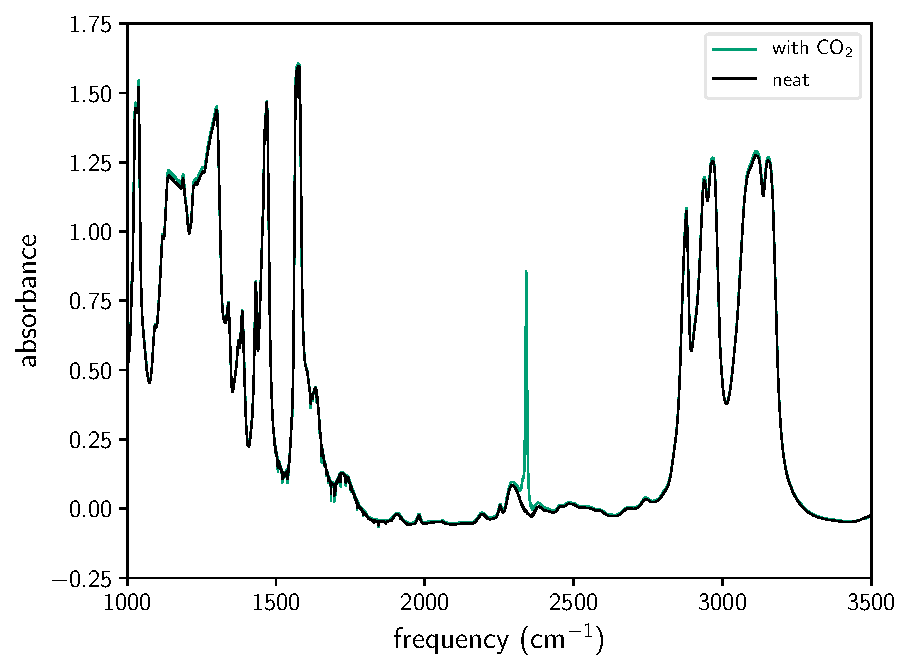
\includegraphics[scale=0.65]{./figures/experimental_spectra_TfO.pdf}
\end{frame}

\begin{frame}
  \centering
  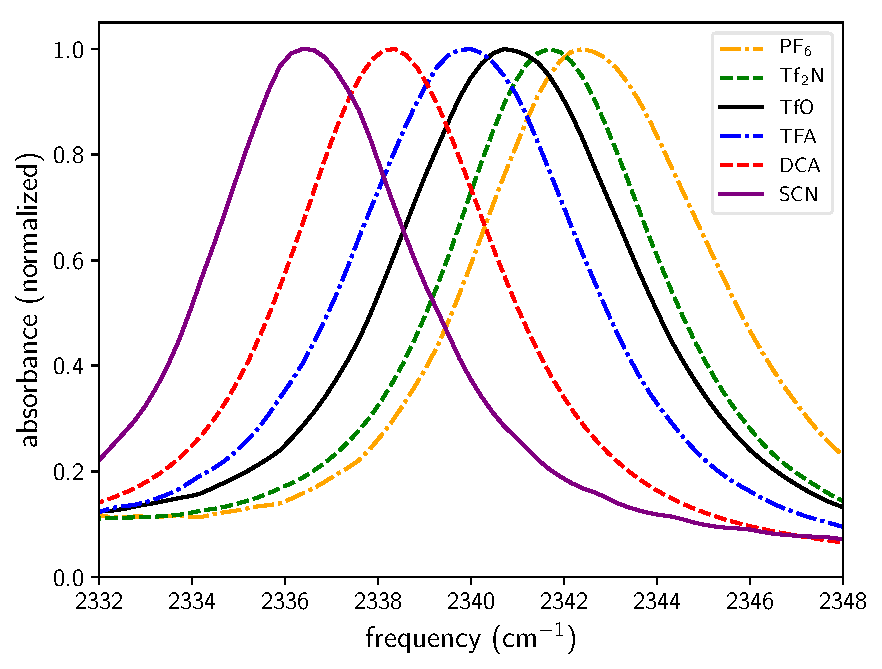
\includegraphics[scale=0.65]{./figures/experimental_spectra_shifting.pdf}
\end{frame}

\begin{frame}
  \centering
  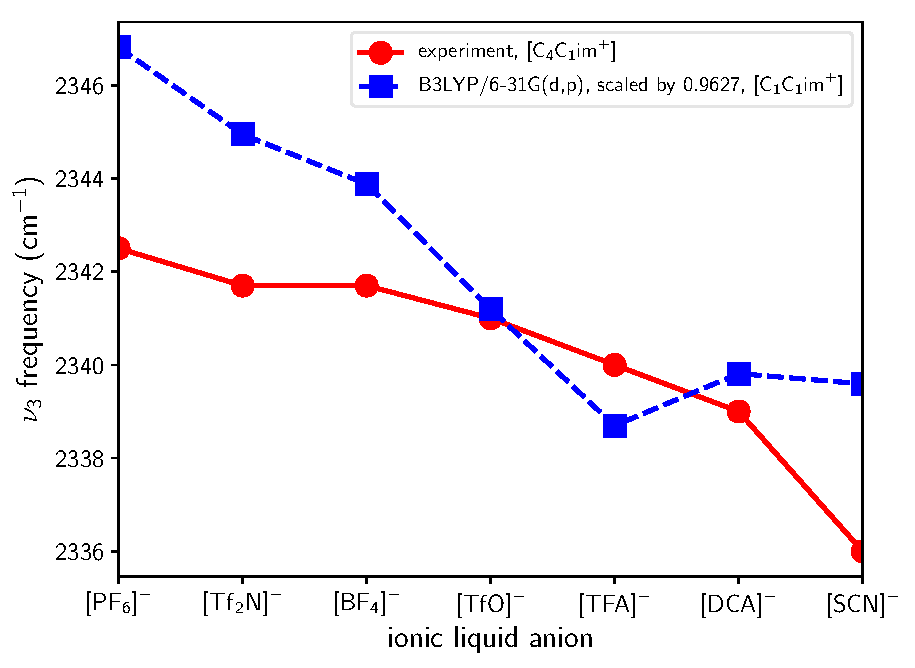
\includegraphics[scale=0.65]{./figures/frequencies_calc_vs_expt1.pdf}
\end{frame}

\begin{frame}
  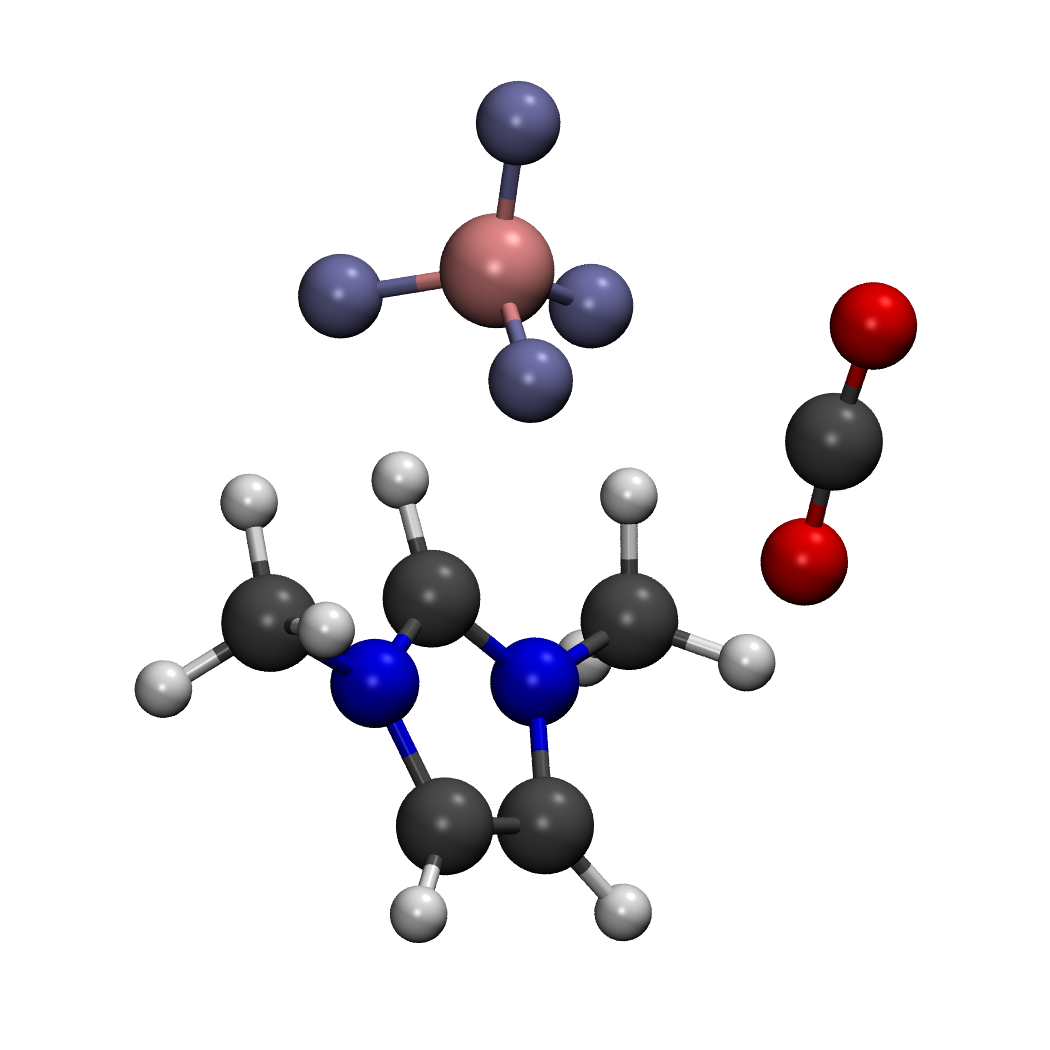
\includegraphics[scale=0.08]{./figures/cluster_BF4.png}
  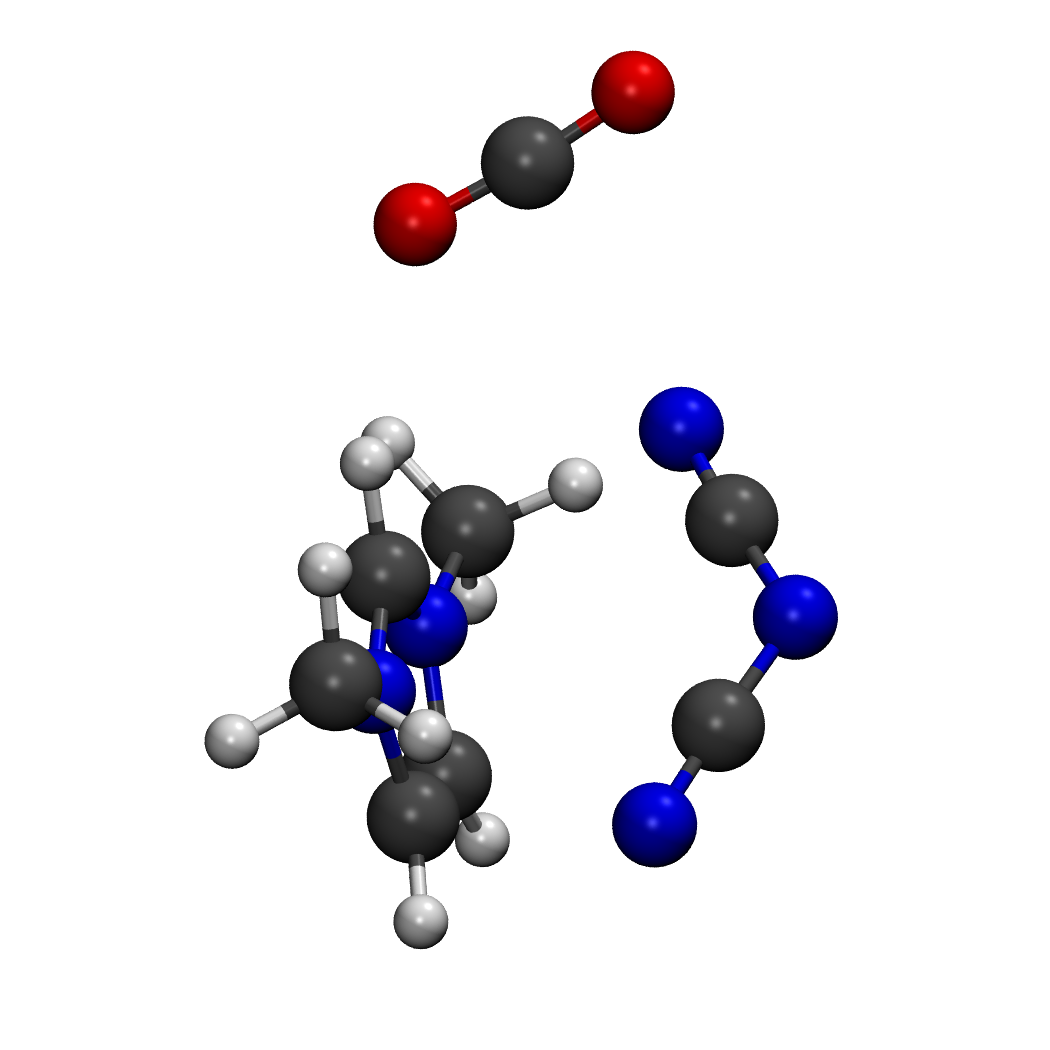
\includegraphics[scale=0.08]{./figures/cluster_DCA.png}
  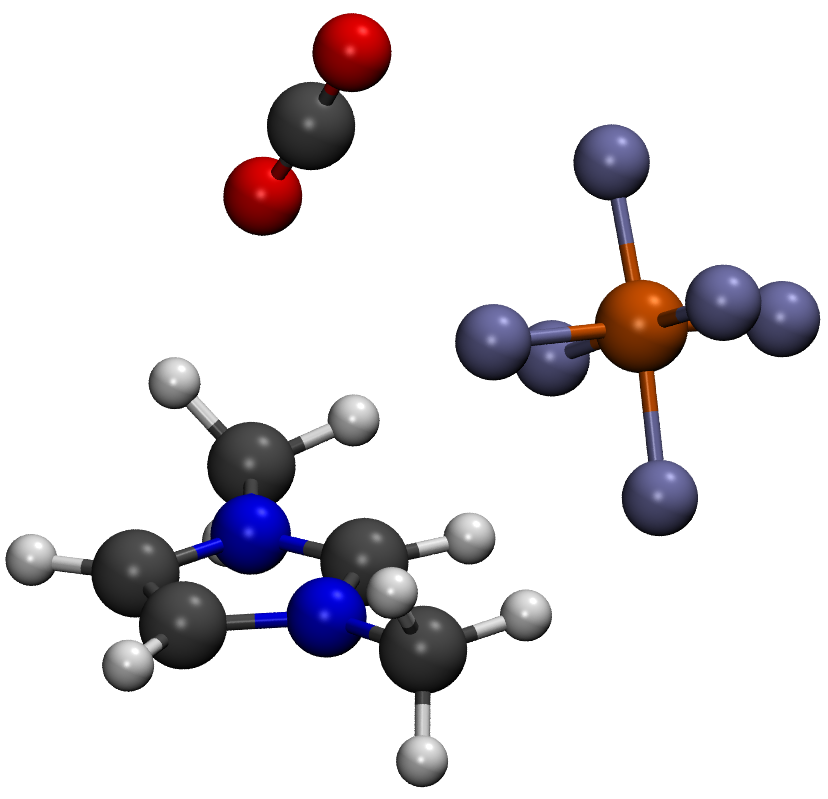
\includegraphics[scale=0.08]{./figures/cluster_PF6.png}
  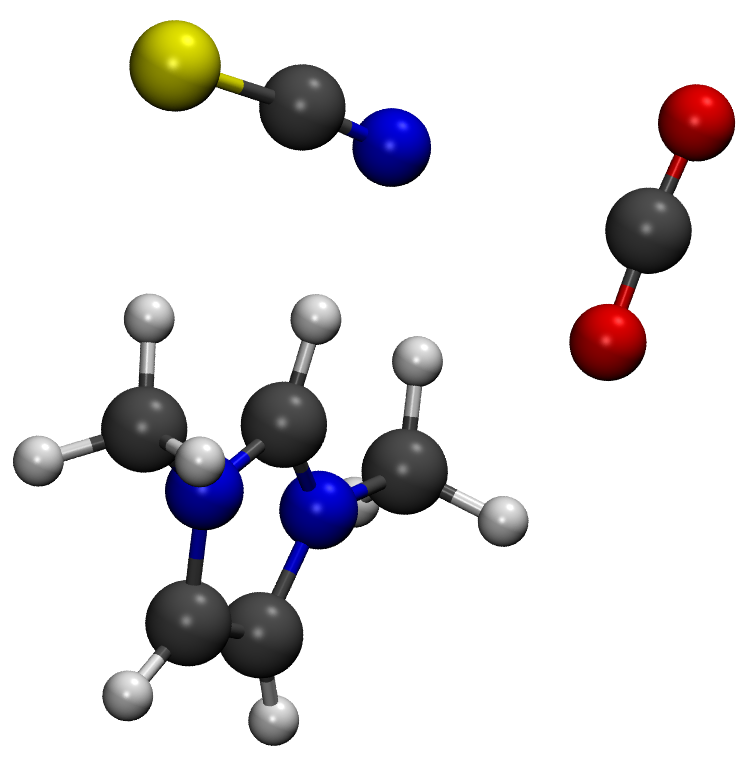
\includegraphics[scale=0.08]{./figures/cluster_SCN.png}
  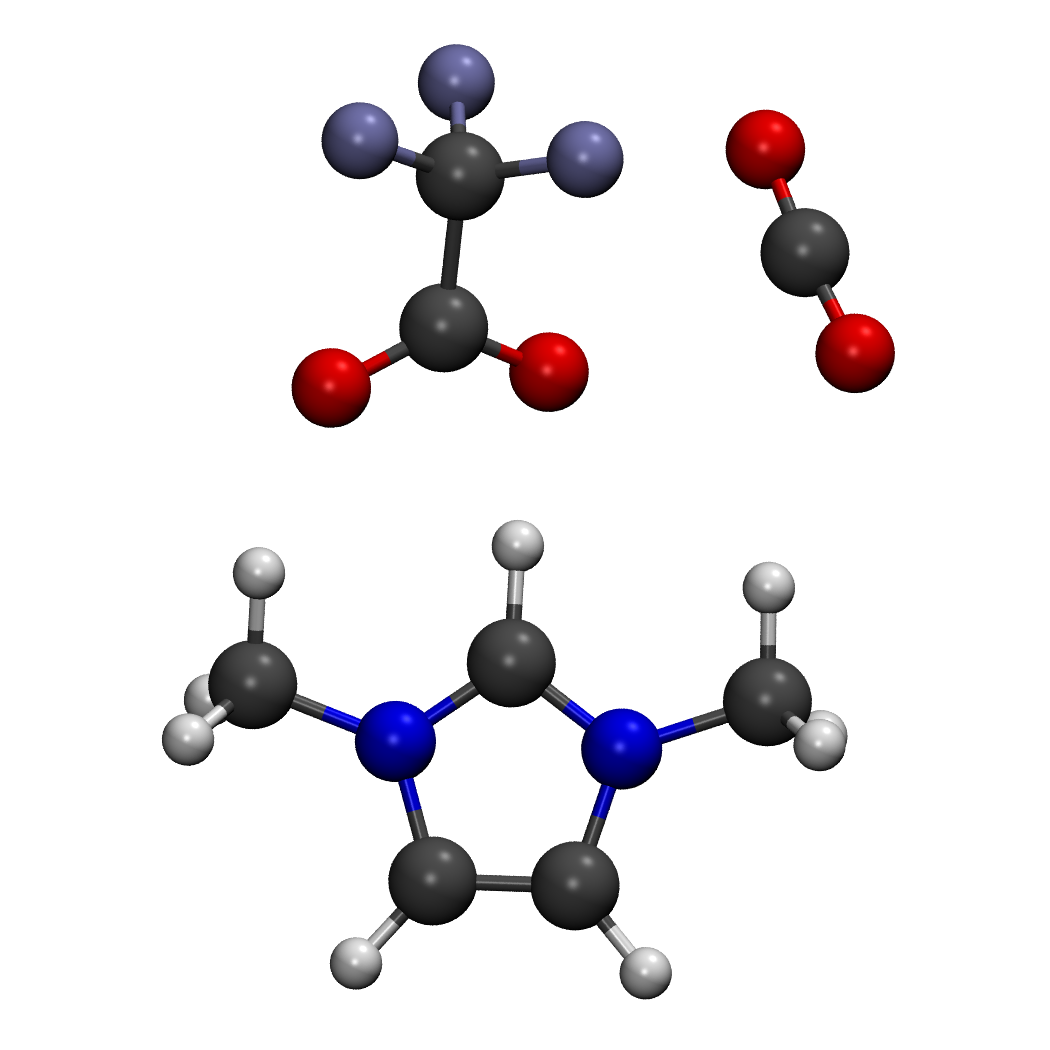
\includegraphics[scale=0.07]{./figures/cluster_TFA.png}
  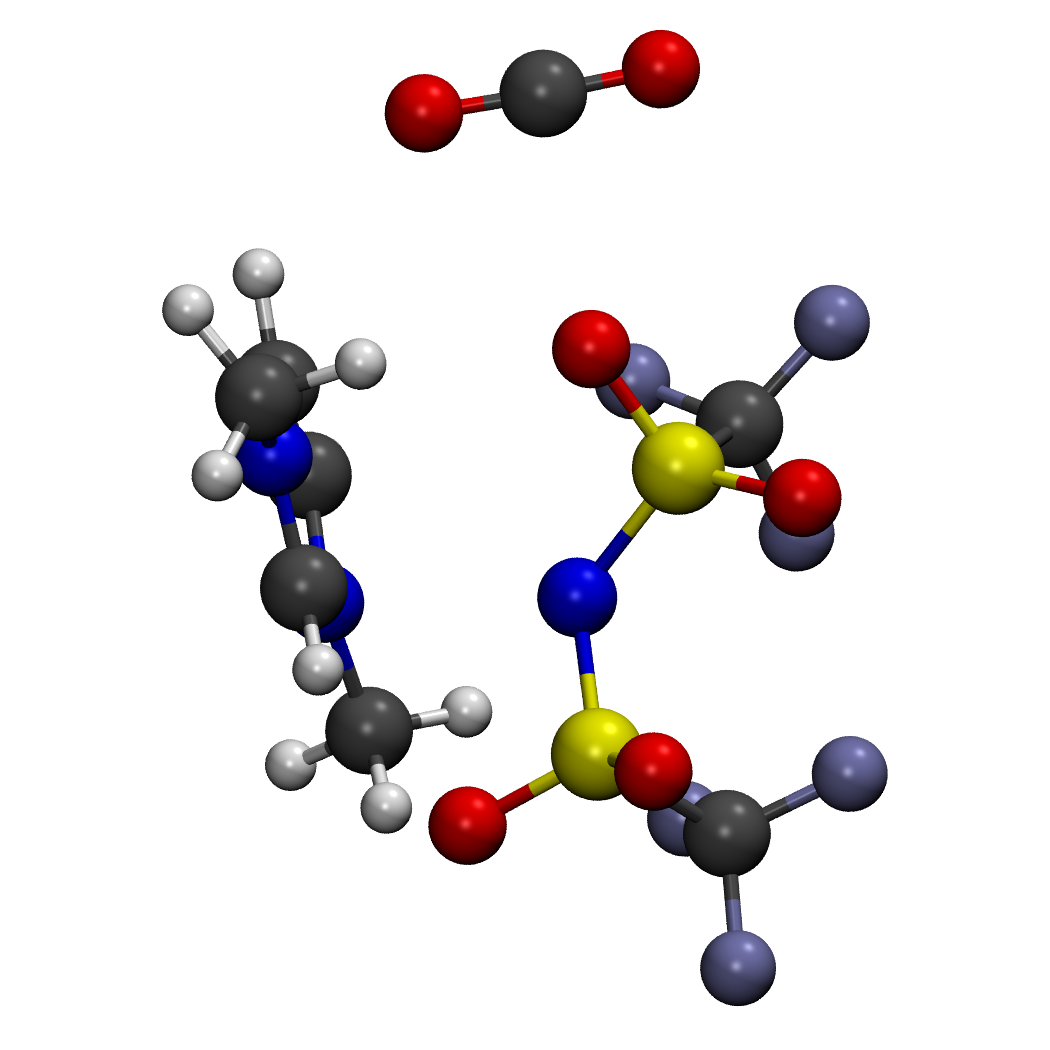
\includegraphics[scale=0.08]{./figures/cluster_Tf2N.png}
  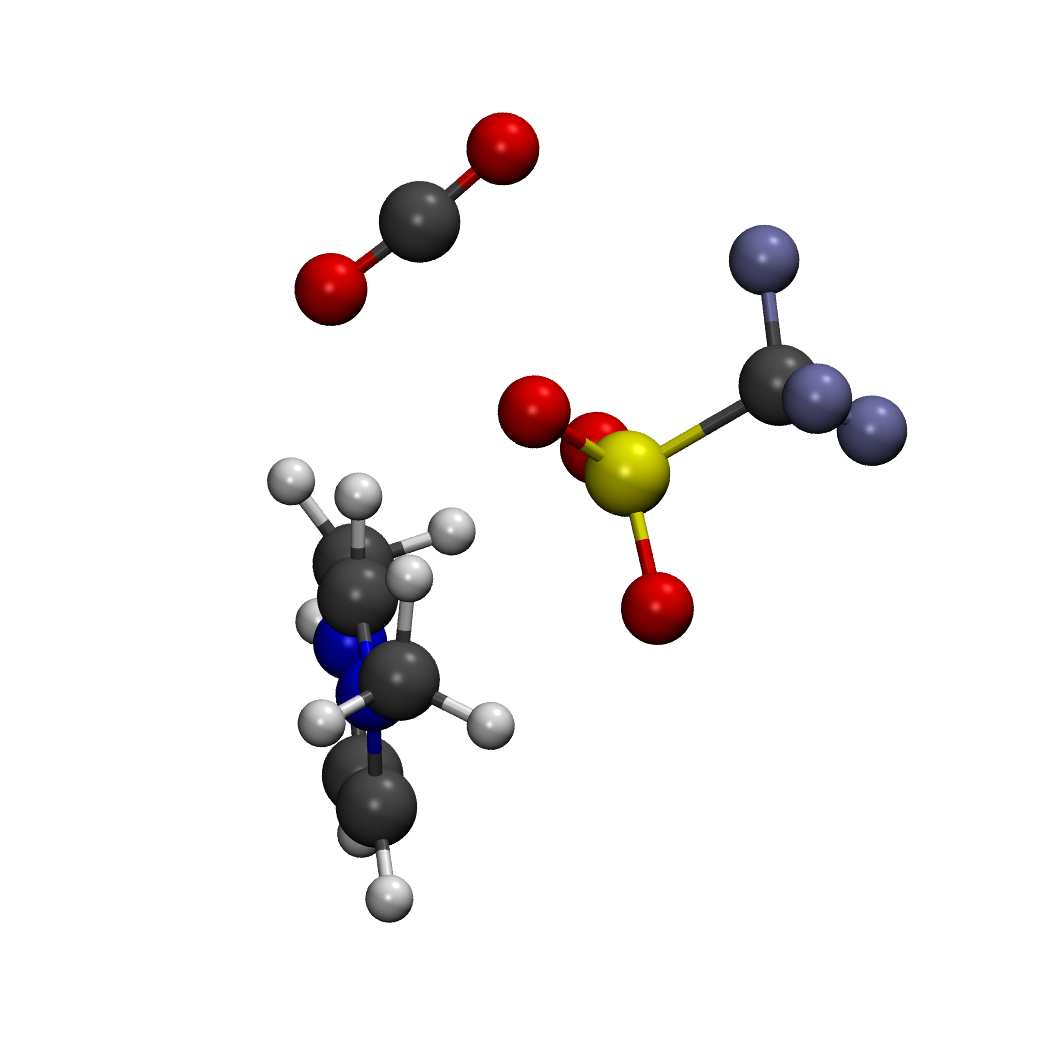
\includegraphics[scale=0.09]{./figures/cluster_TfO.png}
\end{frame}

\begin{frame}
  \frametitle{ALMO-EDA}
  \centering
  \begin{equation*}
    \begin{aligned}
      E_{\text{tot}} &= E_{\text{free}} + \Delta E_{\text{int}} \\
      \Delta E_{\text{int}} &= \Delta E_{\text{gd}} + \Delta E_{\text{frz}} + \Delta E_{\text{pol}} + \Delta E_{\text{CT}}
    \end{aligned}
  \end{equation*}
  \uncover<1->{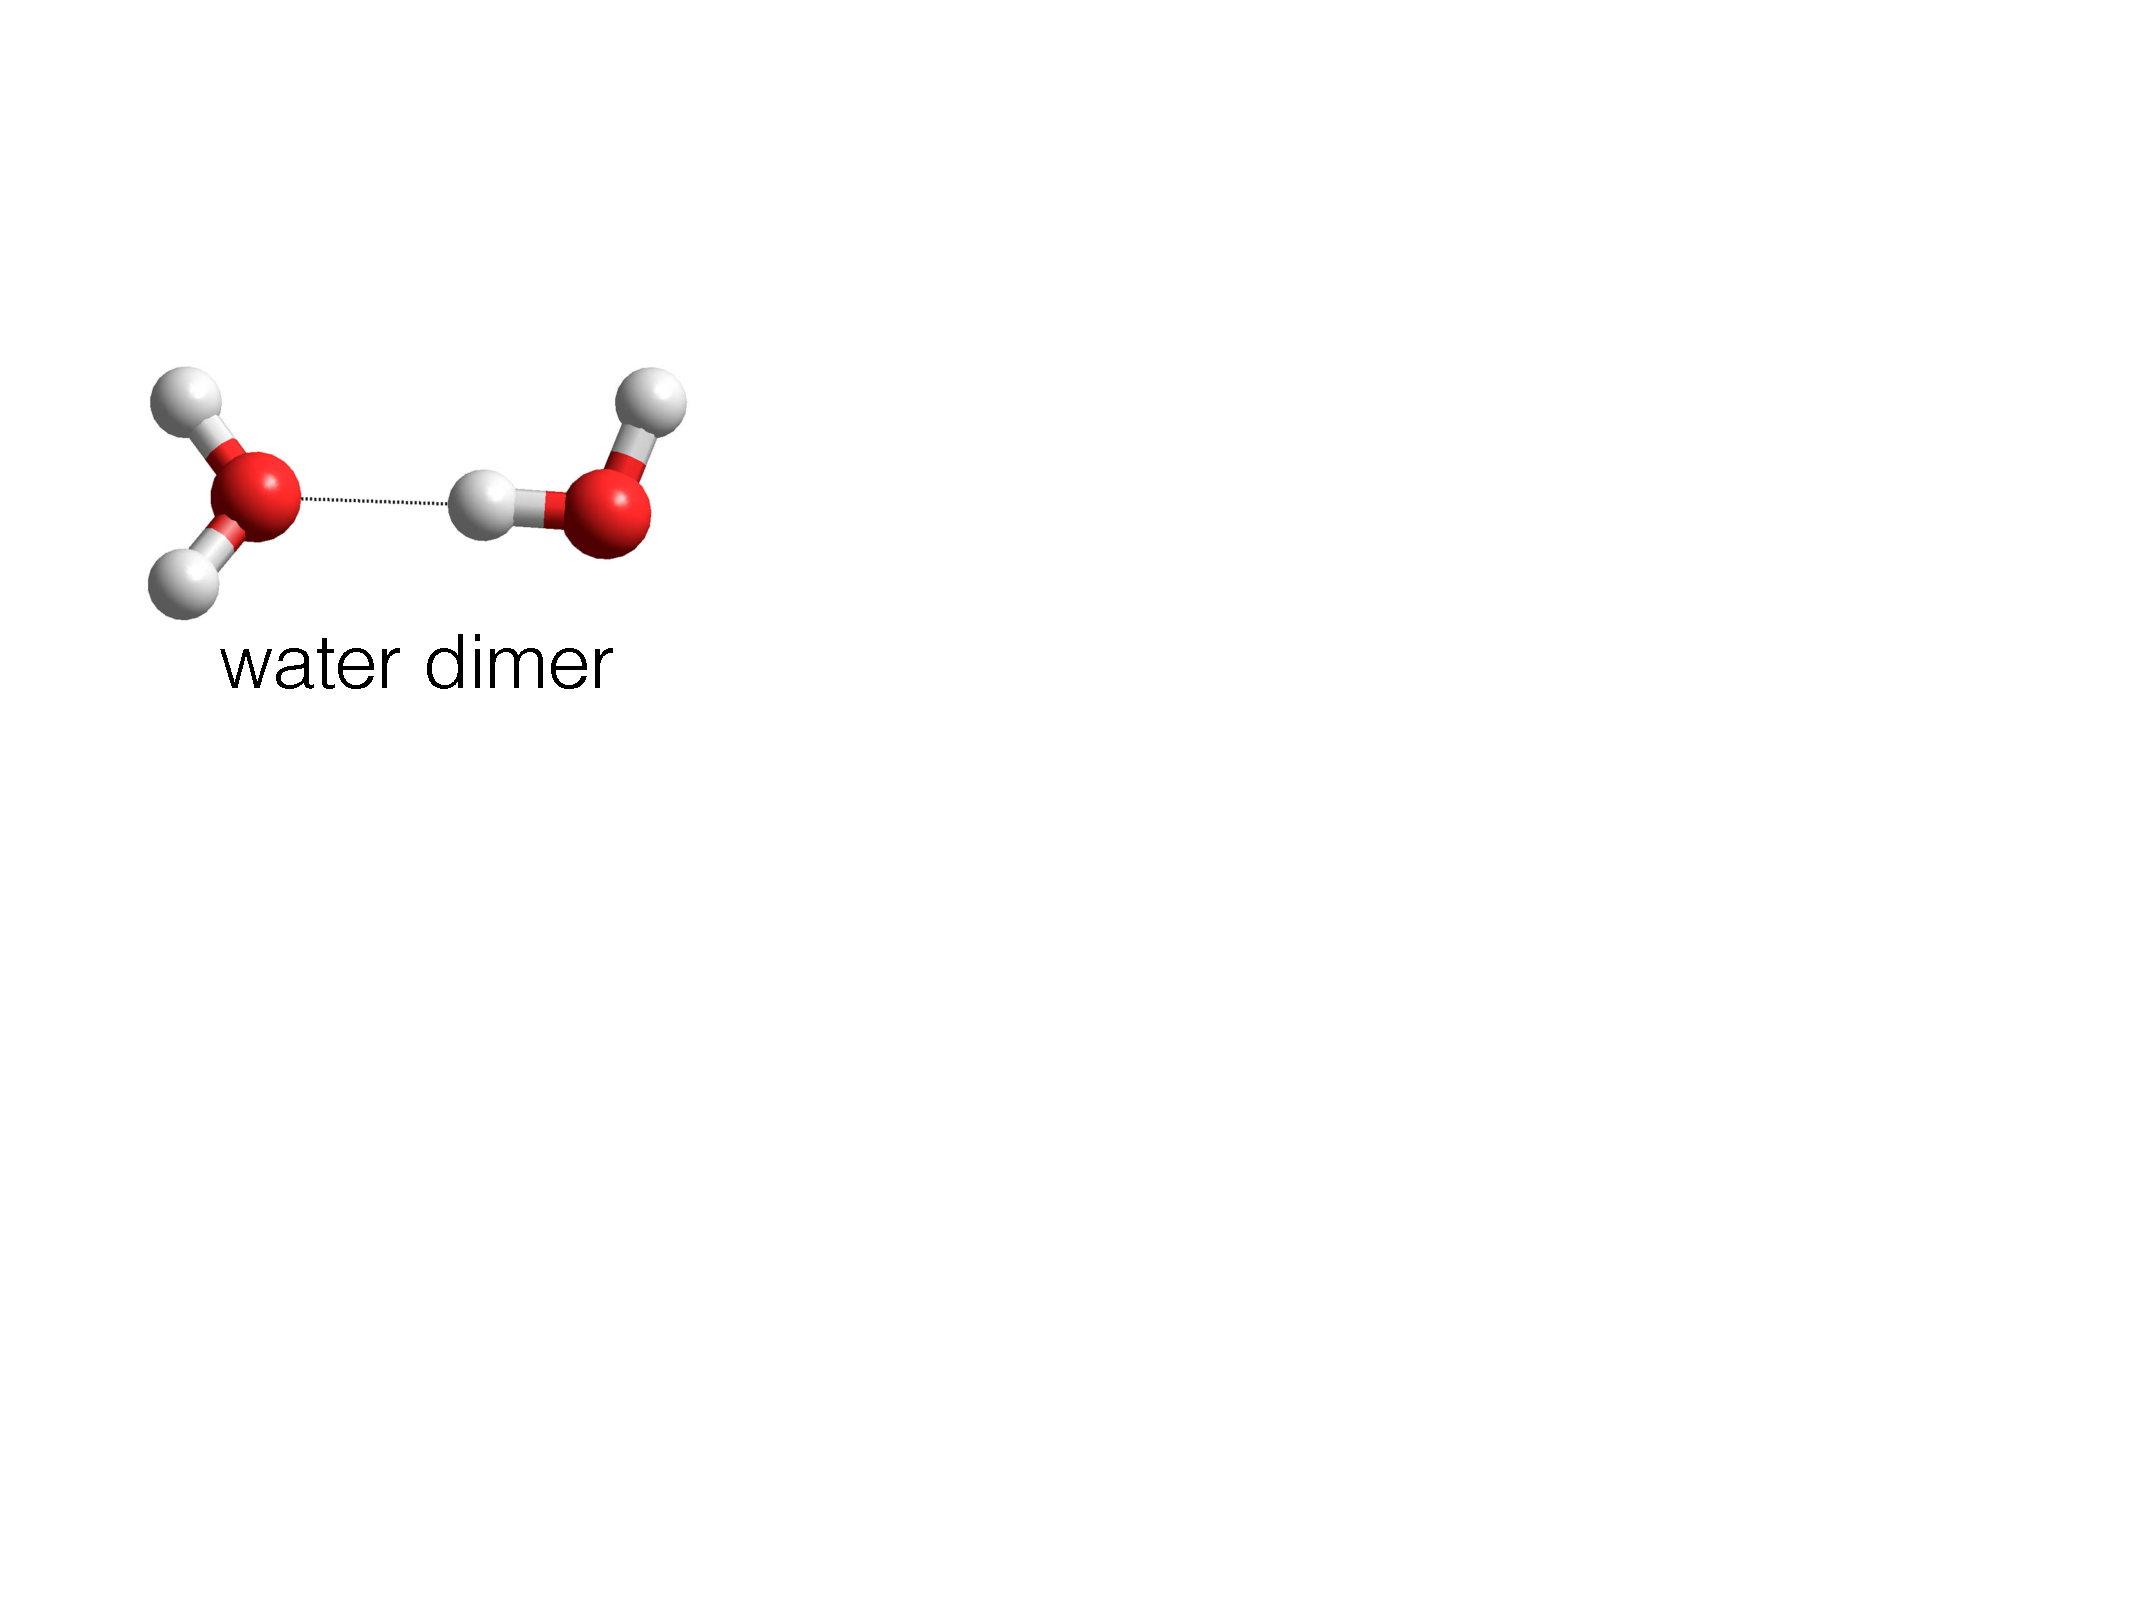
\includegraphics[scale=0.25]{./figures/almo_eda_00.pdf}}
  \uncover<2->{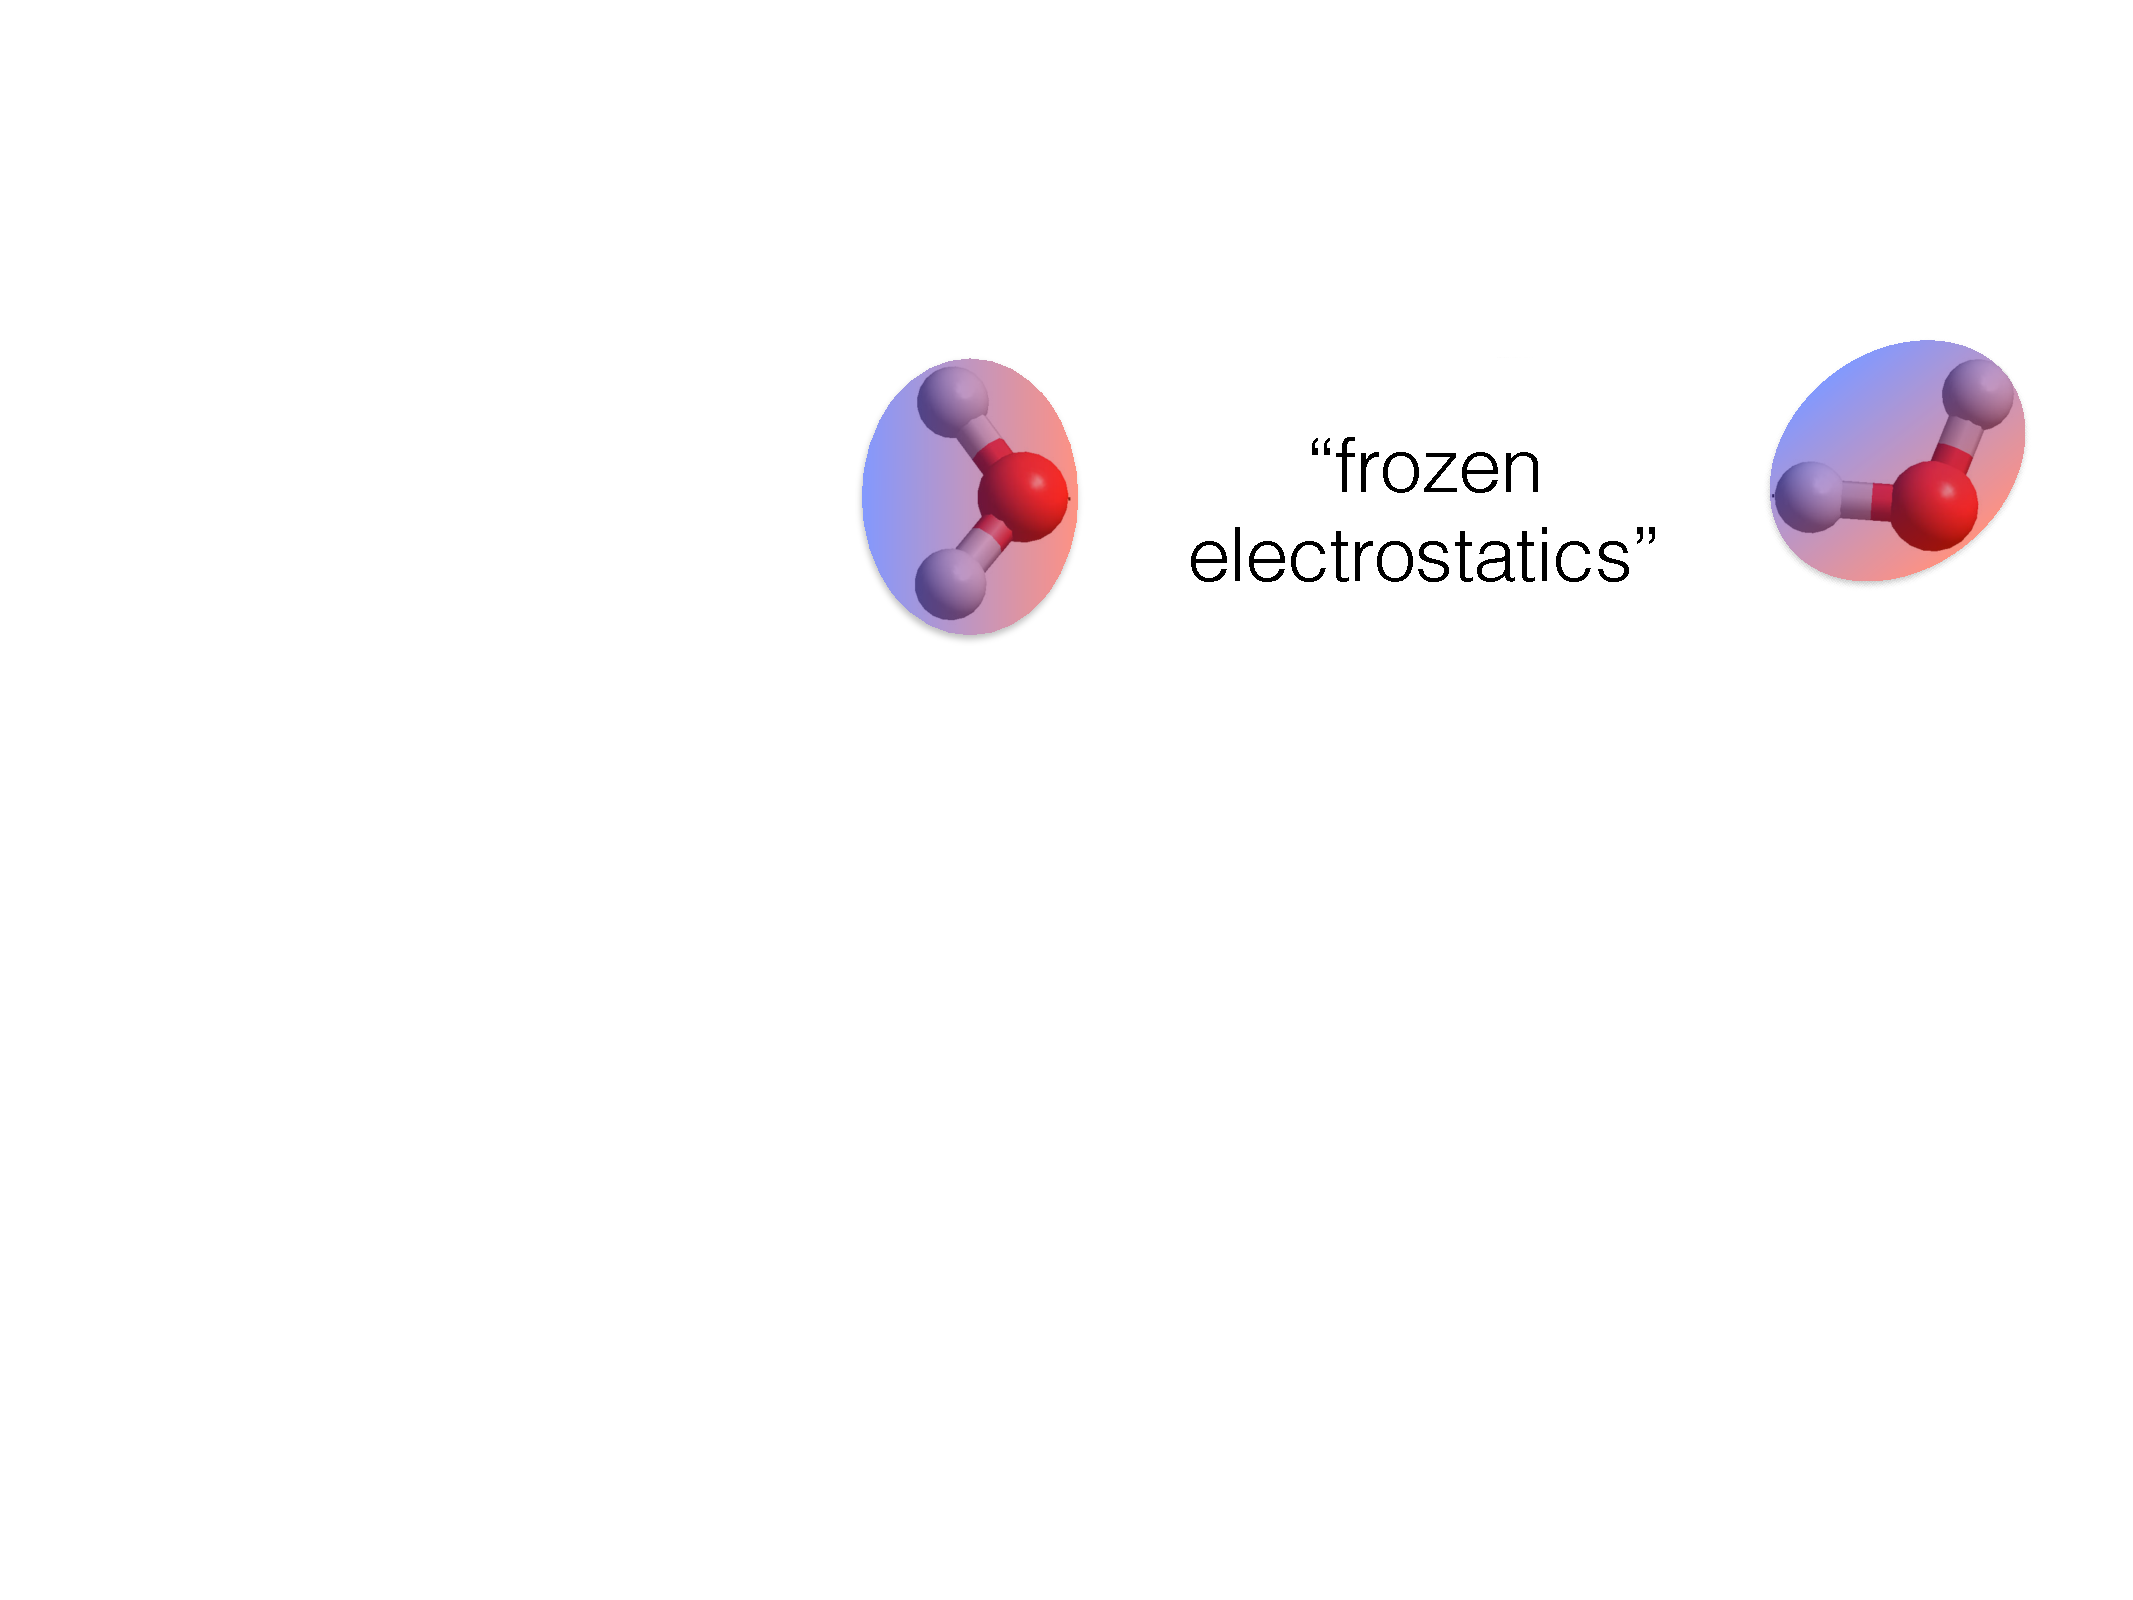
\includegraphics[scale=0.25]{./figures/almo_eda_02_frz.pdf}}
  \uncover<3->{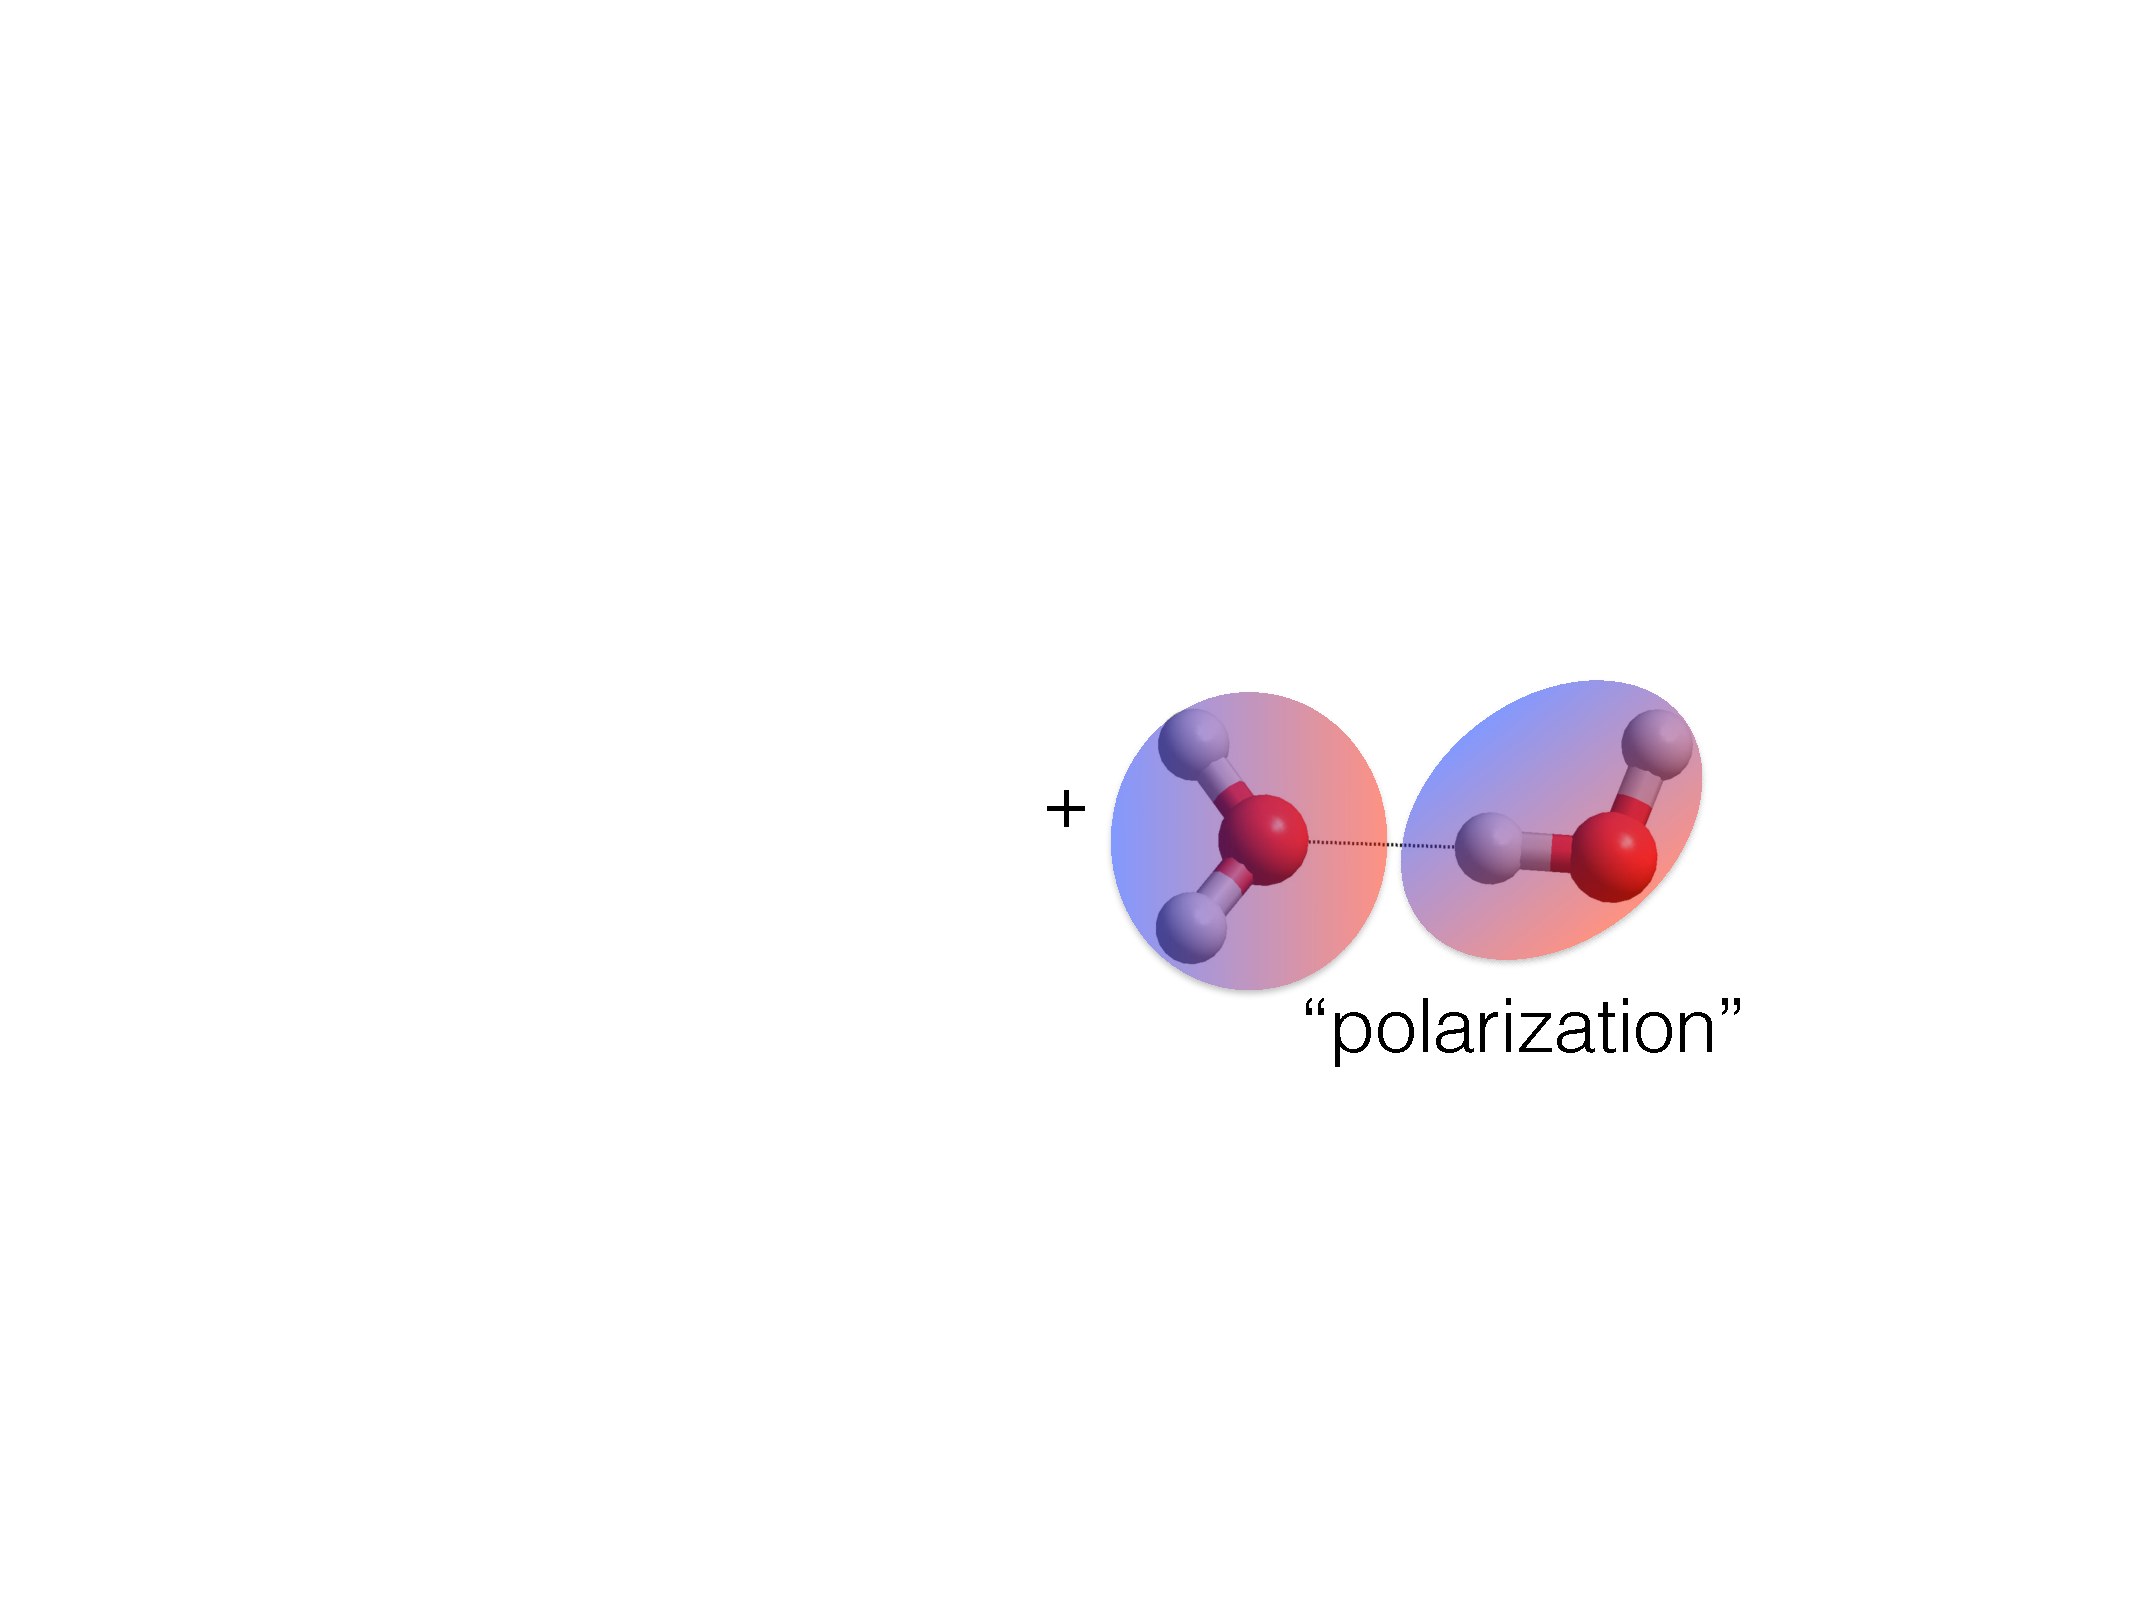
\includegraphics[scale=0.25]{./figures/almo_eda_03_pol.pdf}}
  \uncover<4->{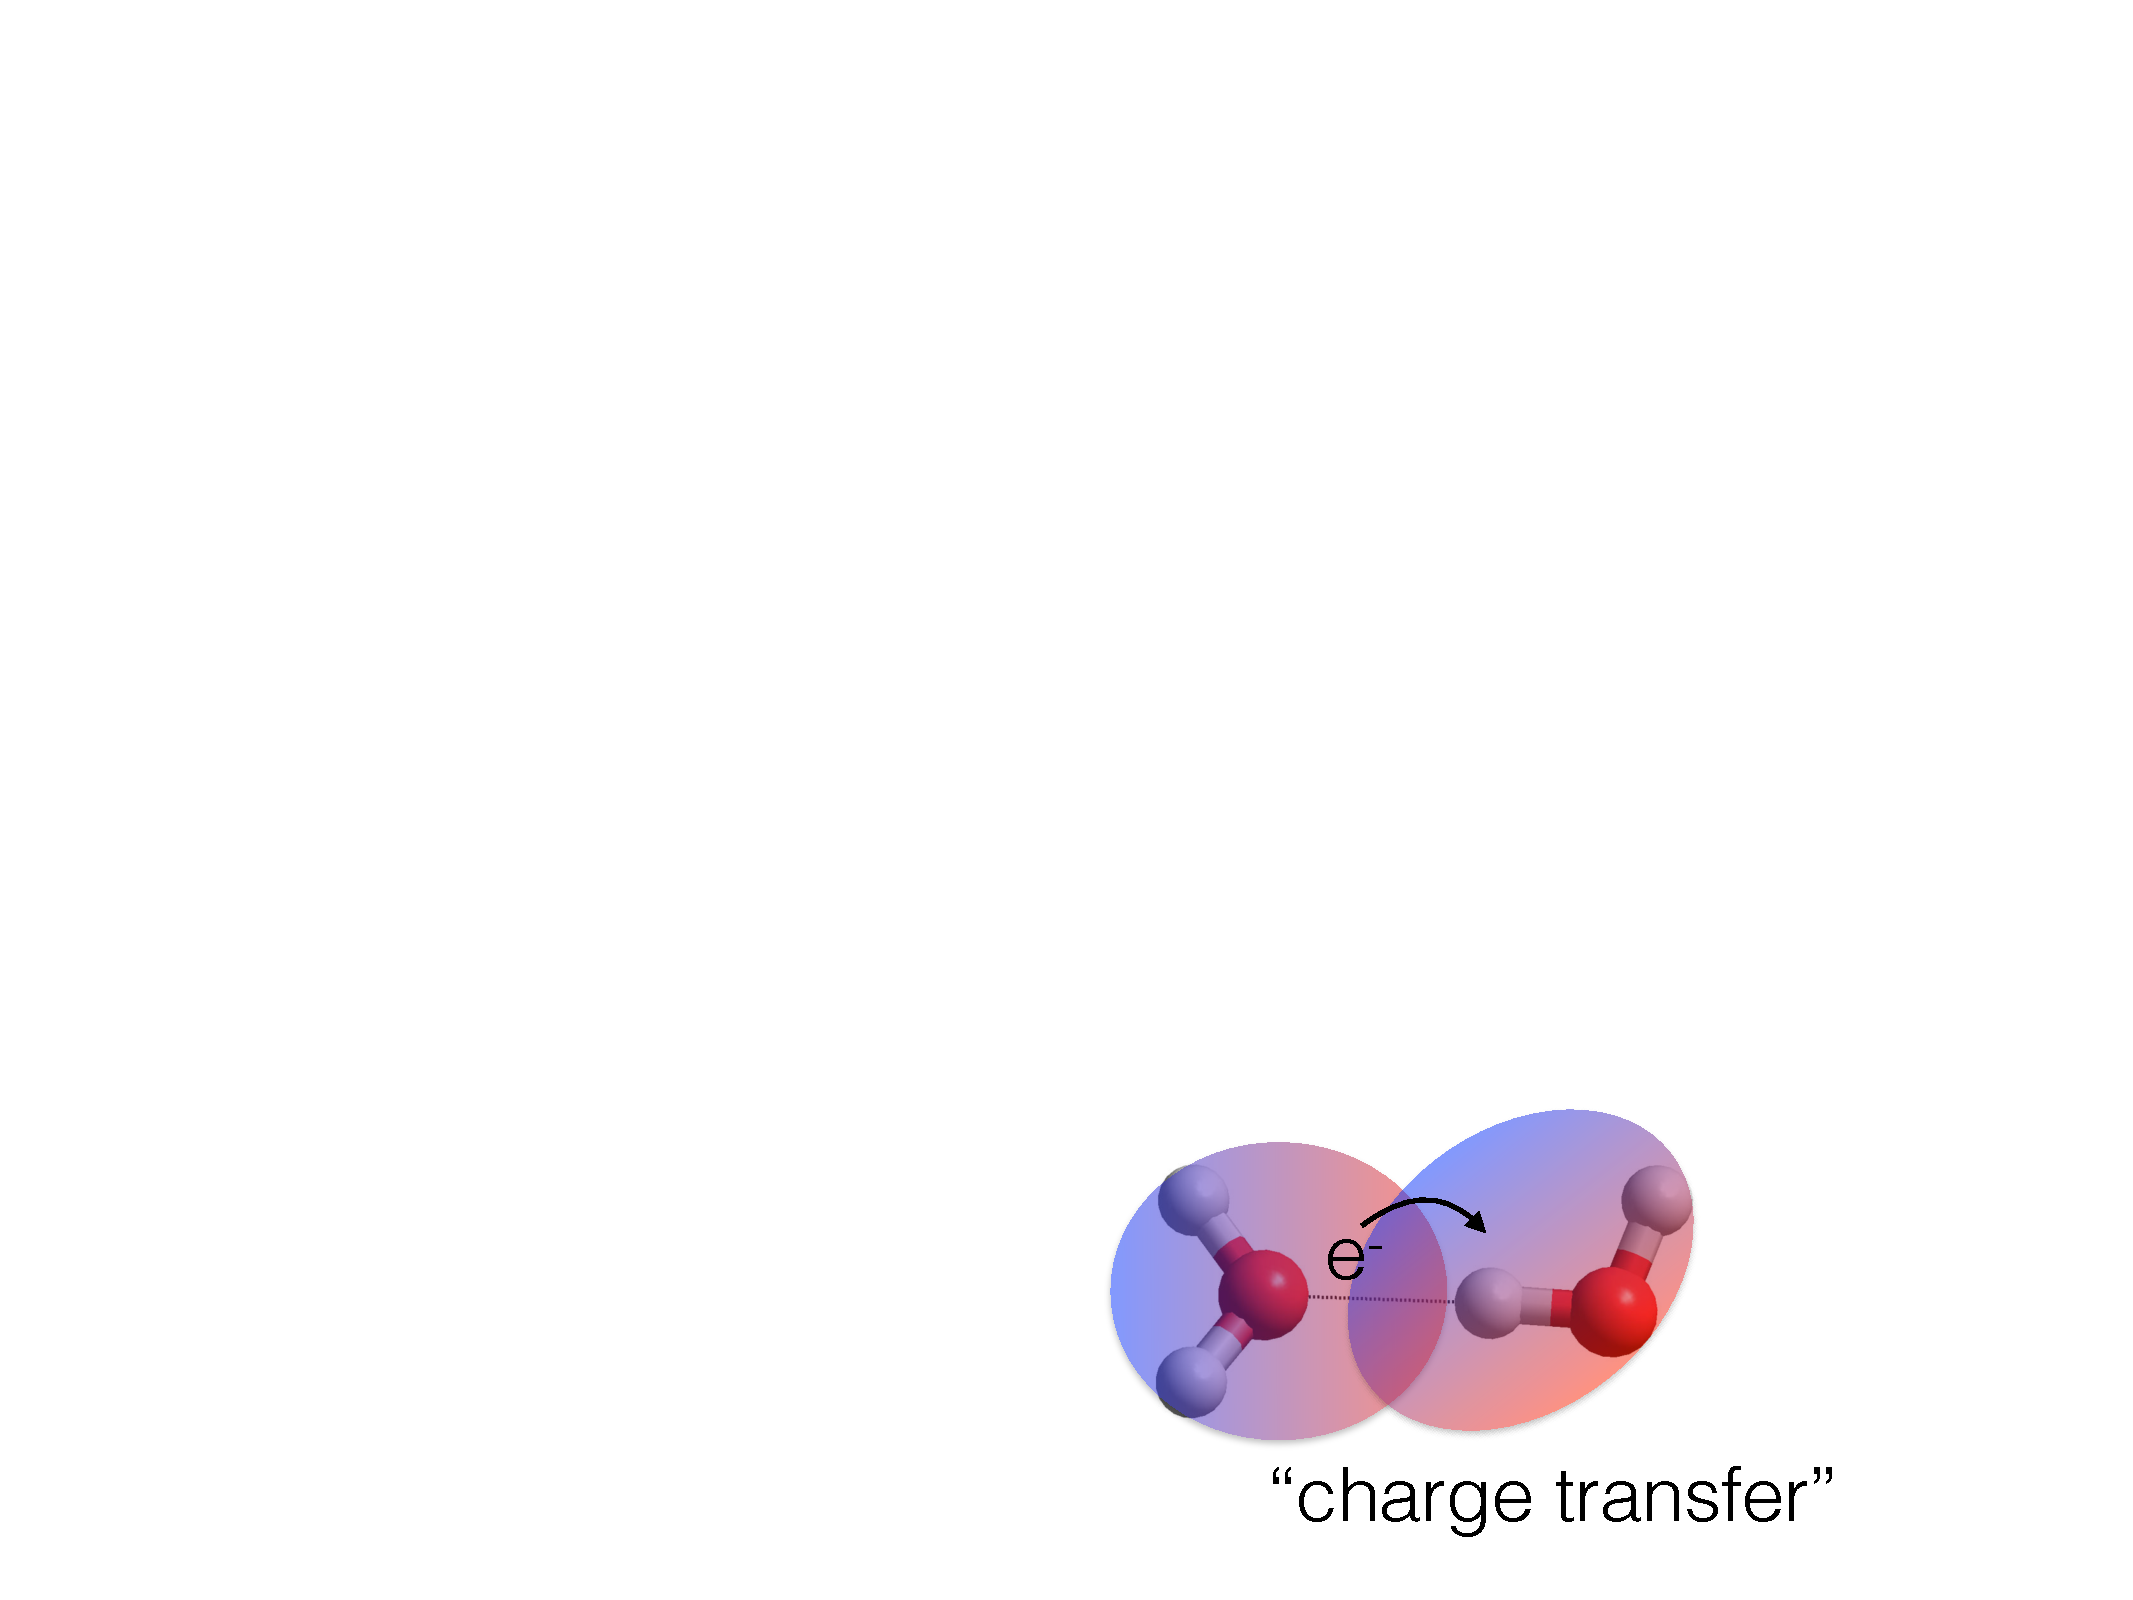
\includegraphics[scale=0.25]{./figures/almo_eda_04_ct.pdf}}
\end{frame}

\begin{frame}
  \frametitle{ALMO-EDA}
  \begin{equation*}
    \begin{aligned}
      \omega_{\text{tot}} &= \omega_{\text{free}} + \Delta \omega_{\text{int}} \\
      \Delta \omega_{\text{int}} &= \Delta \omega_{\text{gd}} + \Delta \omega_{\text{frz}} + \Delta \omega_{\text{pol}} + \Delta \omega_{\text{CT}}
    \end{aligned}
  \end{equation*}
\end{frame}

\begin{frame}
  \uncover<1->{\begin{equation*}
    E_{\text{tot}} = E_{\text{free}} + \Delta E_{\text{gd}} + \Delta E_{\text{frz}} + \Delta E_{\text{pol}} + \Delta E_{\text{CT}}
  \end{equation*}}
  \uncover<2->{\begin{equation*}
    \omega_{\text{tot}} = \omega_{\text{free}} + \Delta \omega_{\text{gd}} + \Delta \omega_{\text{frz}} + \Delta \omega_{\text{pol}} + \Delta \omega_{\text{CT}}
  \end{equation*}}
  \uncover<3->{\begin{equation*}
      \begin{aligned}
        \braket{\braket{\hat{P};\hat{Q}^{\omega}}}_{\text{tot}} = &\braket{\braket{\hat{P};\hat{Q}^{\omega}}}_{\text{free}} + \Delta \braket{\braket{\hat{P};\hat{Q}^{\omega}}}_{\text{gd}} \\
        &+ \Delta \braket{\braket{\hat{P};\hat{Q}^{\omega}}}_{\text{frz}} + \Delta \braket{\braket{\hat{P};\hat{Q}^{\omega}}}_{\text{pol}} + \Delta \braket{\braket{\hat{P};\hat{Q}^{\omega}}}_{\text{CT}}
    \end{aligned}
  \end{equation*}}
\end{frame}

\begin{frame}
  \centering
  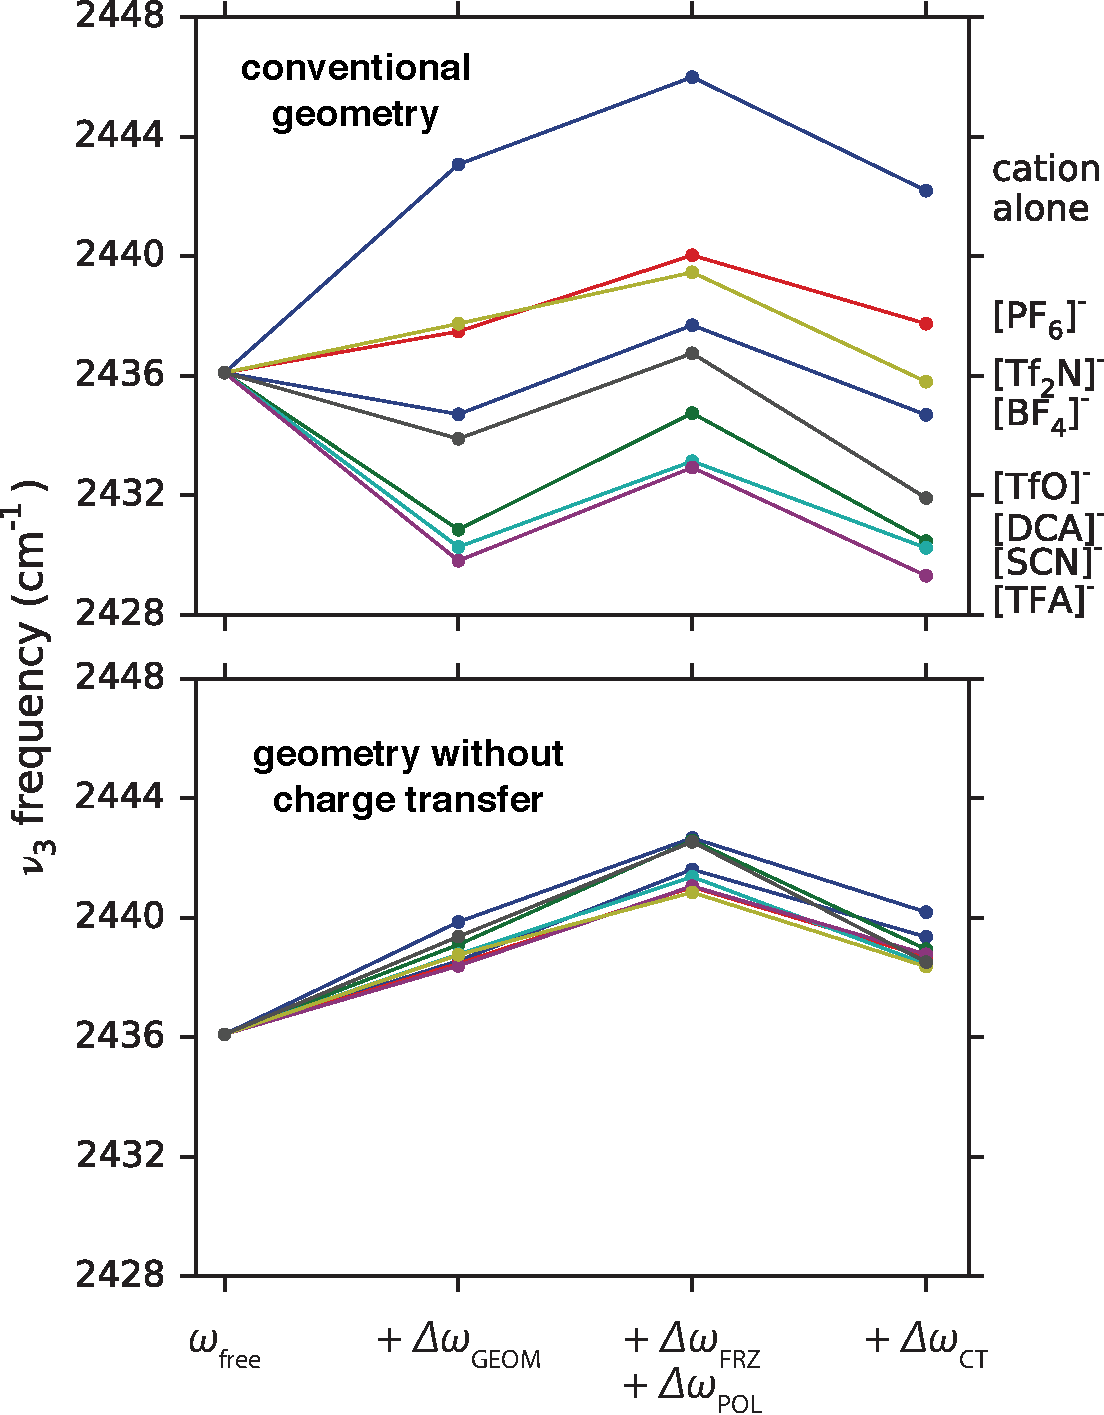
\includegraphics[scale=0.38]{./figures/ionic_liquid_geometry_dependence_on_ct.pdf}
\end{frame}

\begin{frame}
  \centering
  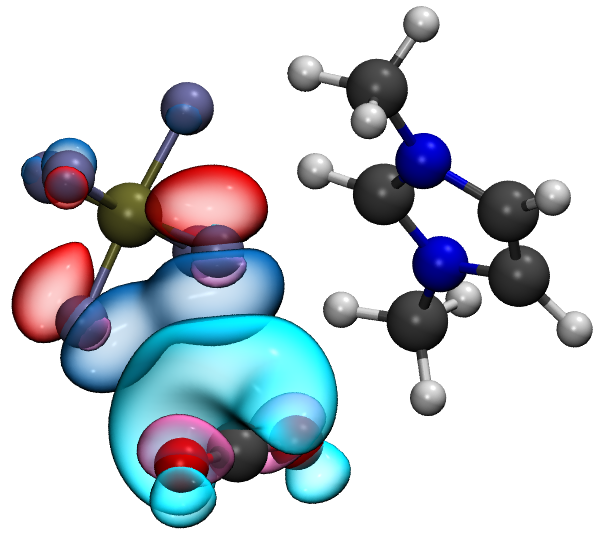
\includegraphics[scale=0.23,natwidth=601,natheight=535]{./figures/PF6.to_CO2.1.png}
  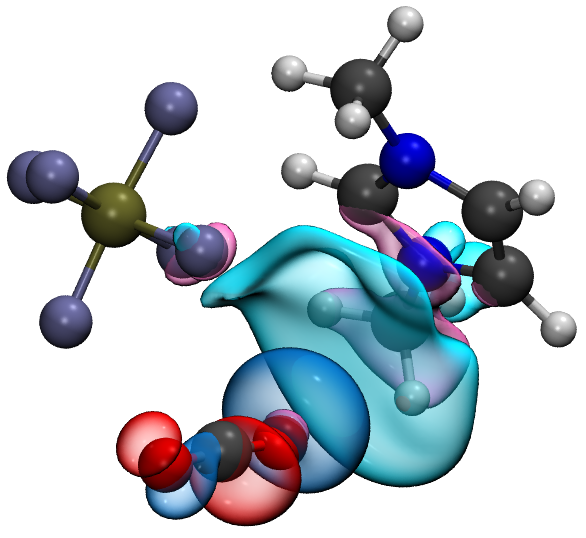
\includegraphics[scale=0.23,natwidth=586,natheight=538]{./figures/PF6.from_CO2.1.png}
\end{frame}

\begin{frame}
  \frametitle{Spectroscopic properties are directly connected to response functions}
  \centering
  \begin{tabular}{ll}
    \toprule
    \textbf{Molecular Property}       & \textbf{Linear Response Function} \\
    \midrule
    polarizability                    & \( \braket{\braket{\hat{\mu};\hat{\mu}}}_{\omega} \) \\
    magnetizability                   & \( \braket{\braket{\hat{m};\hat{m}}}_{0} \) \\
    optical rotation                  & \( \braket{\braket{\hat{\mu};\hat{m}}}_{\omega} \) \\
    electronic circular dichroism     & \( \braket{\braket{\hat{\mu};\hat{m}}}_{\omega_{f}} \) \\
    IR intensities                    & \( \braket{\braket{\hat{\mu};\partial\hat{H}_{0}/\partial R}}_{\omega} \) \\
    NMR spin-spin coupling constants  & \( \braket{\braket{\hat{h}_{\text{SD}};\hat{h}_{\text{SD}}}}_{0} \), \\
                                      & \( \braket{\braket{\hat{h}_{\text{FC}};\hat{h}_{\text{FC}}}}_{0} \), \\
                                      & \( \braket{\braket{\hat{h}_{\text{PSO}};\hat{h}_{\text{PSO}}}}_{0} \) \\
    NMR chemical shifts               & \( \braket{\braket{\hat{l}_{O};\hat{h}_{\text{PSO}}}}_{0} \) \\
    EPR \textit{g}-tensor             & \( \braket{\braket{\hat{l}_{O};\hat{h}_{\text{SOC}}}}_{0} \) \\
    \bottomrule
  \end{tabular}
\end{frame}

% \begin{frame}[fragile]
%   \frametitle{An Algorithm For Finding Primes Numbers.}
% \begin{semiverbatim}
% \uncover<1->{\alert<0>{int main (void)}}
% \uncover<1->{\alert<0>{\{}}
% \uncover<1->{\alert<1>{  \alert<4>{std::}vector<bool> is_prime (100, true);}}
% \uncover<1->{\alert<1>{  for (int i = 2; i < 100; i++)}}
% \uncover<2->{\alert<2>{    if (is_prime[i])}}
% \uncover<2->{\alert<0>{      \{}}
% \uncover<3->{\alert<3>{        \alert<4>{std::}cout << i << " ";}}
% \uncover<3->{\alert<3>{        for (int j = i; j < 100;}}
% \uncover<3->{\alert<3>{             is_prime [j] = false, j+=i);}}
% \uncover<2->{\alert<0>{      \}}}
% \uncover<1->{\alert<0>{  return 0;}}
% \uncover<1->{\alert<0>{\}}}
% \end{semiverbatim}

%   \visible<4->{Note the use of \alert{\texttt{std::}}.}
% \end{frame}

% \begin{frame}
% \end{frame}


\begin{frame}
  \frametitle{Thank you}
  \scriptsize
  \begin{enumerate}
  \item \fullcite{Berquist2014}
  \item \fullcite{Shao2015}
  \item \fullcite{Brinzer2015}
  \item \fullcite{Daly2016}
  \item \fullcite{Berquist2017}
  \item \fullcite{Brinzer2017}
  \item \fullcite{Smith2018}
  \item \fullcite{Berquist2018}
  \item \fullcite{Jakubek2018}
  \end{enumerate}
\end{frame}

\end{document}
